\documentclass[italian,a4paper,11pt]{article}

% path to figure folder
\graphicspath{{figs/}}

\newtheorem{lem}{Lemma}[section]
\newtheorem{definizione}{Definizione}[section]
\newtheorem{teorema}{Teorema}[section]
\newtheorem{pro}{Proposizione}[section]
\newtheorem{cor}{Corollario}[section]
\declaretheoremstyle[
spaceabove=6pt, spacebelow=6pt,
headfont=\normalfont\bfseries,
notefont=\mdseries, notebraces={(}{)},
bodyfont=\normalfont,
postheadspace=1em,
qed=,
]{exercise_style}
\declaretheorem[style=exercise_style, name=Esempio, numberwithin=section]{example}
\declaretheorem[style=exercise_style, name=Esercizio, 
numberwithin=section]{exercise}
\declaretheorem[style=exercise_style, name=Problema,
numberwithin=subsection]{problem}
\declaretheorem[style=exercise_style, name=Osservazione, 
numberwithin=section]{observation}

% abbreviated labels lowercase c
\crefname{lem}{Lem.}{Lemm.}
\crefname{definizione}{Def.}{Def.ni}
\crefname{teorema}{Teo.}{Teo.mi}
\crefname{pro}{Prop.}{Propp.}
\crefname{cor}{Cor.}{Corr.}
% non-abbreviated labels uppercase C
\Crefname{lem}{Lemma}{Lemmi}
\Crefname{definizione}{Definizione}{Definizioni}
\Crefname{teorema}{Teorema}{Teoremi}
\Crefname{pro}{Proposizione}{Proposizioni}
\Crefname{cor}{Corollario}{Corollari}

% turns all (hyperlinked) references black [default is blue]
\hypersetup{
	linktoc=all,
	colorlinks=true,
	linkcolor=black
}

% imports math shorthand notation
\declaretheoremstyle[
spaceabove=6pt, spacebelow=6pt,
headfont=\normalfont\bfseries\itshape,
notefont=\mdseries, notebraces={(}{)},
bodyfont=\normalfont,
postheadspace=1em,
qed=,
]{exercise_style}

\declaretheoremstyle[
spaceabove=6pt, spacebelow=6pt,
postheadspace=1em,
qed=,
]{theorem_style}

\declaretheoremstyle[
spaceabove=6pt, spacebelow=6pt,
postheadspace=1em,
qed=,
]{axiom_style}

\declaretheorem[name=Teorema,numberwithin=section]{theorem}
\declaretheorem[name=Lemma,sibling=theorem]{lemma}
\declaretheorem[name=Proposizione,sibling=theorem]{proposition}
\declaretheorem[name=Corollario,sibling=theorem]{corollary}
\declaretheorem[name=Paradosso,sibling=theorem]{paradox}
\declaretheorem[style=axiom_style,name=Assioma,sibling=theorem]{axiom}
\declaretheorem[name=Definizione,numberwithin=section]{definition}
\declaretheorem[style=exercise_style,name=Esempio,numberwithin=section]{example}
\declaretheorem[style=exercise_style,name=Esercizio,numberwithin=section]{exercise}
\declaretheorem[style=exercise_style,name=Osservazione,numberwithin=section]{remark}

%\renewcommand\qedsymbol{Deh, per forza!}

%\newcommand{\abs}[1]{{\left|#1\right|}}
%\newcommand{\norm}[1]{{\|#1\|}}
\DeclareMathOperator{\Imaginarypart}{Im}
\renewcommand{\Im}{\Imaginarypart}
\DeclareMathOperator{\Realpart}{Re}
\renewcommand{\Re}{\Realpart}

% greek letters
\newcommand{\eps}{\varepsilon}
\renewcommand{\phi}{\varphi}

% blackboard letters
\newcommand{\CC}{\mathbb C}
\newcommand{\HH}{\mathbb H}
\newcommand{\II}{\mathbb{I}}
\newcommand{\KK}{\mathbb K}
\newcommand{\NN}{\mathbb N}
\newcommand{\QQ}{\mathbb Q}
\newcommand{\RR}{\mathbb R}
\newcommand{\TT}{\mathbb T}
\newcommand{\ZZ}{\mathbb Z}

% Upright d in math mode (for differentials).
% -> d
\newcommand{\ud}{\mathrm{d}}

% Differential.
% -> dx
\newcommand{\diff}[1][x]{\,\ud{#1}}

% Base command for defining derivatives.
% -> df/dx or d^kf/dx^k
\newcommand{\basederivative}[4][]{%
  \displaystyle%
  \ifx\\#1\\\frac{#4#2}{#4#3}%
  \else%
  \frac{#4^#1#2}{#4#3^#1}%
  \fi%
}

% Total derivative.
% -> df/dx(x) or d^kf/dx^k(x)
\newcommand{\td}[4][]{%
  \basederivative[#1]{#2}{#3}{\ud}%
  \ifx\\#4\\%
  \else%
  \mkern-4mu\left(#4\right)%
  \fi%
}

% Partial derivative.
% -> df/dx(x) or d^kf/dx^k(x)
\newcommand{\pd}[4][]{%
  \basederivative[#1]{#2}{#3}{\partial}%
  \ifx\\#4\\%
  \else%
  \mkern-4mu\left(#4\right)%
  \fi%
}

% Tilde under variables v_~
\DeclareMathAccent{\wtilde}{\mathord}{largesymbols}{"65}
\newcommand{\utld}[1]{\underaccent{\wtilde}{#1}}

\newcommand{\ds}{\displaystyle}

% Image of a map
\DeclareMathOperator{\Ima}{Im}

\declaretheoremstyle[
spaceabove=6pt, spacebelow=6pt,
headfont=\normalfont\bfseries\itshape,
notefont=\mdseries, notebraces={(}{)},
bodyfont=\normalfont,
postheadspace=1em,
qed=,
]{exercise_style}

\declaretheoremstyle[
spaceabove=6pt, spacebelow=6pt,
postheadspace=1em,
qed=,
]{theorem_style}

\declaretheoremstyle[
spaceabove=6pt, spacebelow=6pt,
postheadspace=1em,
qed=,
]{axiom_style}

\declaretheorem[name=Teorema,numberwithin=section]{theorem}
\declaretheorem[name=Lemma,sibling=theorem]{lemma}
\declaretheorem[name=Proposizione,sibling=theorem]{proposition}
\declaretheorem[name=Corollario,sibling=theorem]{corollary}
\declaretheorem[name=Paradosso,sibling=theorem]{paradox}
\declaretheorem[style=axiom_style,name=Assioma,sibling=theorem]{axiom}
\declaretheorem[name=Definizione,numberwithin=section]{definition}
\declaretheorem[style=exercise_style,name=Esempio,numberwithin=section]{example}
\declaretheorem[style=exercise_style,name=Esercizio,numberwithin=section]{exercise}
\declaretheorem[style=exercise_style,name=Osservazione,numberwithin=section]{remark}

%\renewcommand\qedsymbol{Deh, per forza!}

%\newcommand{\abs}[1]{{\left|#1\right|}}
%\newcommand{\norm}[1]{{\|#1\|}}
\DeclareMathOperator{\Imaginarypart}{Im}
\renewcommand{\Im}{\Imaginarypart}
\DeclareMathOperator{\Realpart}{Re}
\renewcommand{\Re}{\Realpart}

% greek letters
\newcommand{\eps}{\varepsilon}
\renewcommand{\phi}{\varphi}

% blackboard letters
\newcommand{\CC}{\mathbb C}
\newcommand{\HH}{\mathbb H}
\newcommand{\II}{\mathbb{I}}
\newcommand{\KK}{\mathbb K}
\newcommand{\NN}{\mathbb N}
\newcommand{\QQ}{\mathbb Q}
\newcommand{\RR}{\mathbb R}
\newcommand{\TT}{\mathbb T}
\newcommand{\ZZ}{\mathbb Z}

% Upright d in math mode (for differentials).
% -> d
\newcommand{\ud}{\mathrm{d}}

% Differential.
% -> dx
\newcommand{\diff}[1][x]{\,\ud{#1}}

% Base command for defining derivatives.
% -> df/dx or d^kf/dx^k
\newcommand{\basederivative}[4][]{%
  \displaystyle%
  \ifx\\#1\\\frac{#4#2}{#4#3}%
  \else%
  \frac{#4^#1#2}{#4#3^#1}%
  \fi%
}

% Total derivative.
% -> df/dx(x) or d^kf/dx^k(x)
\newcommand{\td}[4][]{%
  \basederivative[#1]{#2}{#3}{\ud}%
  \ifx\\#4\\%
  \else%
  \mkern-4mu\left(#4\right)%
  \fi%
}

% Partial derivative.
% -> df/dx(x) or d^kf/dx^k(x)
\newcommand{\pd}[4][]{%
  \basederivative[#1]{#2}{#3}{\partial}%
  \ifx\\#4\\%
  \else%
  \mkern-4mu\left(#4\right)%
  \fi%
}

% Tilde under variables v_~
\DeclareMathAccent{\wtilde}{\mathord}{largesymbols}{"65}
\newcommand{\utld}[1]{\underaccent{\wtilde}{#1}}

\newcommand{\ds}{\displaystyle}

% Image of a map
\DeclareMathOperator{\Ima}{Im}


\geometry{a4paper, left=30mm, right=30mm, top=30mm, bottom=30mm}


\title{Esercizi di Geometria Differenziale\\ del 2 Ottobre}
\author{Marco Romagnoli (578061)\thanks{svolti insieme a Bernardo Tomelleri (587829)}}
\date{\today}


\begin{document}
\maketitle

\section*{Esercizio 1.3}
\begin{proof}[Svolgimento]
Sia $f:X\rightarrow Y$ una funzione continua tra spazi topologici e sia $A\subseteq Y$ un intorno di $f(x)$, con $x\in X$ generico.
Per definizione di intorno esiste un $V$ aperto in $Y$ tale che $f(x) \in V \subseteq A$ e data la continuità di $f$ si ha che $f^{-1}(V)$ è a sua volta un aperto in $X$.
Inoltre si ha che $x\in f^{-1}(V) \subseteq f^{-1}(A)$, quindi $f^{-1}(A)$ è un intorno di $x$ e dato che è stato preso un punto generico, vale $\forall x \in X$.\\
Sia ora $f:X\rightarrow Y$ tale che $\forall x \in X$ la controimmagine di un intorno $A$ di $f(x)$ è un intorno di $x$. 
Quindi esistono $U$ aperto in $X$ tale che $x \in U \subseteq f^{-1}(A)$ e $V$ aperto in $Y$ tale che $f(x) \in V \subseteq A$. In particolare prendo $U$ e $V$ in modo tale che siano i più grandi possibili nei rispettivi intorni, cioè che ogni altro aperto che contiene $x$ o $f(x)$ sia contenuto in essi. Da questo si vede che l'immagine di $\left( f^{-1}(A) \setminus U\right) \coloneqq B$ deve essere contenuta in $A$ ma non è a sua volta un intorno di $f(x)$. 
Quindi deve essere $V=A\setminus f(B)$, da cui $f^{-1}(V) = U$.
 
\end{proof}


\section*{Esercizio 1.5}
\begin{proof}[Svolgimento]
Suppongo che per assurdo che $I = \left[0,1\right]$ non sia connesso e che quindi esistano $U_1, U_2$ aperti in $I$ con le seguenti proprietà:
\begin{enumerate}
\item $U_1 \neq \emptyset , U_2 \neq I$ e viceversa
\item $U_1 \cap U_2 = \emptyset$
\item $U_1 \cup U_2 = I.$  
\end{enumerate}

Questi aperti dovranno essere della forma $U_1 = [0,b)$ e $U_2 = (c,1]$, infatti, se scegliessi degli aperti del tipo $(a,b)$ con $a>0$ potrei semplicemente unirlo all'aperto $[0,a+\epsilon )$, per un certo $\epsilon>0$, e ottenere un aperto più grande, stessa cosa per l'estremo opposto. Inoltre, se anche prendessi l'aperto $(0,1)$, il suo complementare $\{0\}\cup\{1\}$ non sarebbe un aperto in $I$.
Per cui ci sono tre possibilità:
\begin{enumerate}
\item $b>c$ ma allora l'intersezione non sarebbe nulla
\item $b<c$ ma allora esisterebbe un intervallo $[b,c]$ i cui elementi non sono contenuti né in $U_1$ né in $U_2$
\item $b=c \coloneqq x$ ma allora l'elemento $x \notin U_1 \cup U_2$.  
\end{enumerate}

\end{proof}

\section*{Esercizio 1.6}
\begin{proof}[Svolgimento]
Voglio dimostrare che l'insieme $$ X = \left\{(0,y) | y \in [-1,1]\right\} \bigcup \left\{\left(x,\sin{\frac1x}\right)|x>0\right\} := R\cup S $$ è connesso ma non connesso per archi.\\
Si vede subito che i singoli insiemi $R$ e $S$ sono entrambi connessi. Per $R$ la dimostrazione è analoga a quella dell'esercizio $1.5$, mentre per $S$ si può notare che, essendo il grafico di una funzione $f:(0,+\infty)\rightarrow \RR$ continua è connessa per archi (ogni arco è semplicemente una restrizione della funzione stessa). 
In particolare non possono esistere due aperti disgiunti la cui unione è uguale ad $R$, ma se prendessi un aperto in $X$ (che si ottiene intersecando un aperto di $\RR^2$ con $X$ stesso) che contenga tutto $R$, dovrebbe avere intersezione non nulla con $S$, poiché $\sin{(1/x)}$ è ben definita $\forall x>0$, e quindi essere del tipo $$R\cup  \left\{\left(x,\sin{\frac1x}\right)|x \in (0,\epsilon)\right\}.$$
Ma nemmeno $S$ può essere formato da unione di due aperti disgiunti.
%Similmente all'esercizio $1.5$ provo a cercare due possibili aperti disgiunti la cui unione forma $X$.
%Nonostante $X \subset \RR^2$ sia definito come unione di due insiemi, questi non sono aperti in $X$, infatti un aperto in $X$, che si ottiene come intersezione di un aperto di $\RR^2$ con $X$ stesso, che contenga  completamente $R$ deve contenere anche dei punti di $S$, poiché $(0,0)$ è un punto di accumulazione per $S$. 
%Quindi, se ho un aperto del tipo $$U_1 = R\cup  \left\{\left(x,\sin{\frac1x}\right)|x \in (0,\epsilon)\right\}$$ 
%l'altro aperto dovrà essere $$ U_2  \left\{\left(x,\sin{\frac1x}\right)|x>\epsilon \right\}$$ ma $(\epsilon , \sin{1/\epsilon}) \notin U_1 \cup U_2$. 
Quindi $X$ è connesso.\\
Adesso provo a connettere un punto di $R$ con $(1/\pi ,0) \in S$ tramite una curva $\gamma$. 
La lunghezza di $\gamma$ è sicuramente maggiore della lunghezza della curva spezzata $\lambda$ definita come l'unione di tutti i segmenti che collegano uno zero di $\sin{1/x}$, per $x=1/(n\pi)$ all'estremo adiacente, per $x=2/[(2n+1)\pi]$ (\cref{fig}).
\begin{figure}[!htb]
\centering
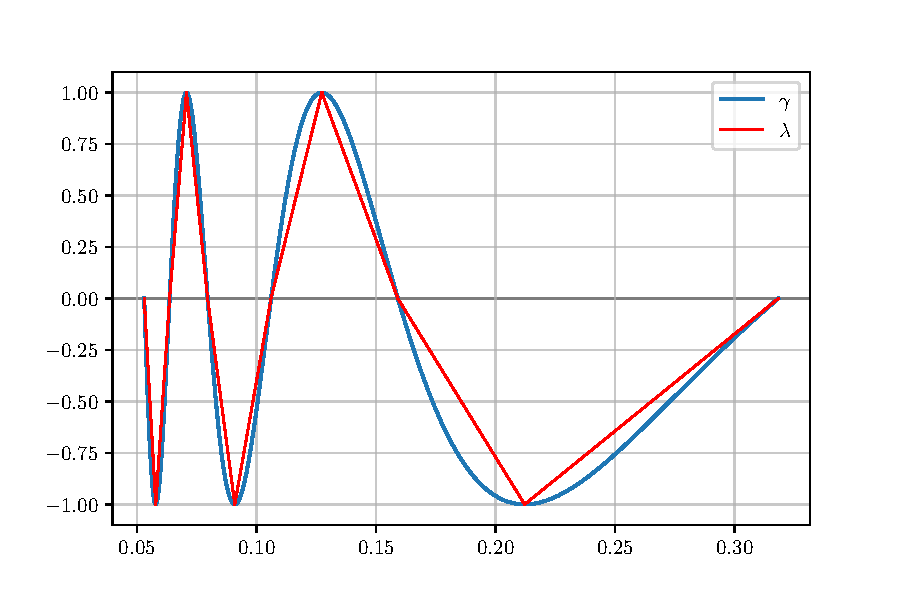
\includegraphics[scale=0.8]{../img/sin1x.pdf}
\caption{Grafici (parziali) di $\gamma$ e $\lambda$.}
\label{fig}
\end{figure}
Si vede che la lunghezza di $\lambda$ è 

\begin{equation*}
l(\lambda) = \sum^{\infty}_{n=1} { \sqrt{\left(\frac{1}{n\pi }-\frac{2}{(2n+1)\pi }\right)^2 + 1} } \geq  \sum^{\infty}_{n=1}1 \longrightarrow \infty . 
\end{equation*}

Allora $\gamma$ ha lunghezza infinita e quindi, in generale, non posso connettere un punto di $R$ ad un punto di $S$ con una curva continua.
\end{proof}


\end{document}
